\noindent 
\begin{homework}{SCARA Robot Mobility Analysis:}
	\newline 
Using the mobility condition, determine and explain why the SCARA robot of Fig 2.5 has the number degrees of freedom that you find.
\end{homework}

\begin{solution}
	We have the following general equation from the mobility condition:
	\begin{align}
	\mathfrak{M} = 6(n - g - 1) + \sum_{i=1}^{g} f_i.
	\label{eq:mobility}
	\end{align}
	%
	where $n$ is the number of links, $g$ is the total number of joints and $f_i$  are the respective relative degrees of freedoms of the individual joints. The SCARA manipulator has three joints with an $RRP$ configuration \ie, $g=3$. These connect four links (including the end-effector) so that $n = 4$. Each of the joints have $f_i=1$. Plugging these into \eqref{eq:mobility}, we find that
	%
	\begin{align}
	\mathfrak{M} = 6(4-3-1) + \sum_{i=1}^3 f_i = 3
	\end{align}
	%
	Hence, the SCARA manipulator is a 3DOF robot.
\end{solution}

\begin{homework}{Parallel Robot Mechanism Analysis}
\newline 
With the \textit{{Gr\"ubler-Kutzbach's} mobility condition} that we have learned, analyze the mobility criteria of the mechanism of \autoref{fig:para_mech}. Hint: This mechanism is made up of two chains: chains $A_3\, B_3\, B_1\, A_1$ and $A_2\, B_2\, B_4\, A_4$, and there is a fixed distance between the $U$-joints, $A_2\, A_3$ as well as $A_1, A_4$.

\begin{figure}[tbph!]
	\centering
	\begin{tabular}{@{}c@{}c@{}}
		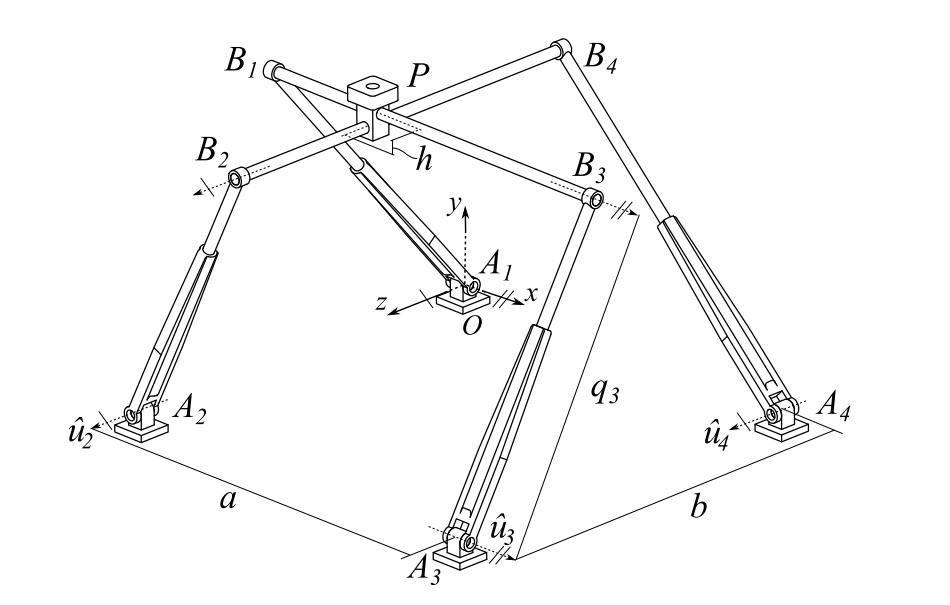
\includegraphics[width=0.50\linewidth ,height=0.4\columnwidth]{../lec_notes/figures/parallel_translational.png} \,\,
		&
		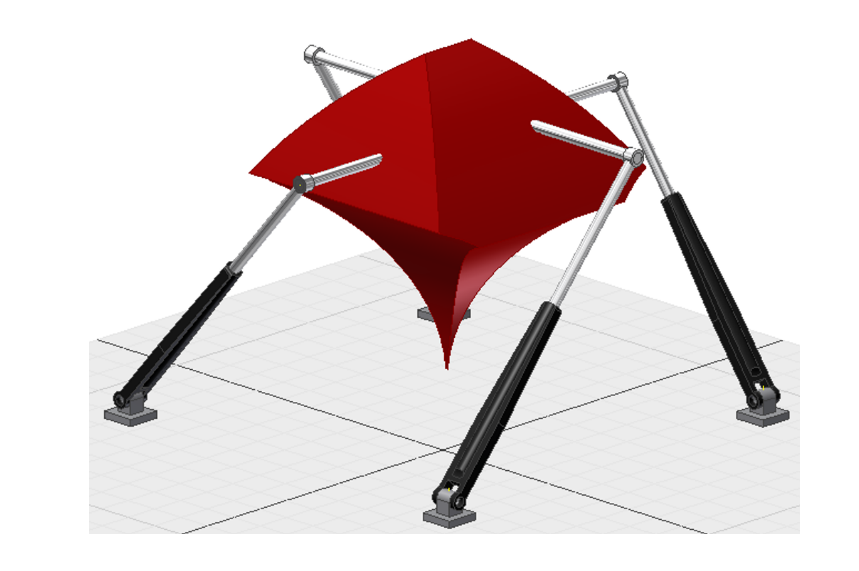
\includegraphics[width=0.48\columnwidth,height=0.4\columnwidth]{../lec_notes/figures/parallel_translational_workspace.png}
	\end{tabular}
	\caption{\textit{Left}: A Parallel Planar Robot Mechanism. \textit{Right:} Workspace of the mechanism.}
	\label{fig:para_mech}
\end{figure}
\end{homework}

\begin{solution}This robot has four RPRP-type kinematic chains. Three of these chains have their prismatic pair closest to the base; they serve as active joints. The fourth kinematic chain is completely passive. Points $B_1$ and $B_2$ are connected by a rod, which is perpendicular to the rod that connects points $B_2$ and $B_4$. Both rods are connected to the moving platform by prismatic joints, which are separated from each other by a vertical offset $h$. Point $P = (P_x,P_y, P_z)$ is the interconnecting point for all the chains on the mobile platform and the top rods. Notice that the rotational axes of the revolute joints \ie, $\bm{\hat{u}}_i$ are parallel to the x-axes of joints 1 and 3; also, they are parallel to the z-axis for joints 2 and 4. 
	
	There are many ways of solving this mobility problem. However, note that this mechanism has multiple closed loops and care must be taken when using the formulas we have introduced in our notes. Here, I will be using Gogu's method as proposed in ~\cite{Gogu}. It decomposes the mechanism into the different closed loops in order to properly analyze the mobility constraint. The mobility of the mechanism is 
	%
	\begin{align}
	\mathfrak{M} = \sum_{i=1}^{g} f_i - r
	\end{align}
	%
	with $r$ being the number of joint parameters that lose independence after closing the loops of the mechanism. We define $r$ as 
	%
	\begin{align}
	r = \sum_{j=1}^{k}SH_j - SF  r_l
	\end{align}
	%
	where $k$ is the number of closed-loops in the mechanism, $SH_j$ is the connectivity of the $j$'th closed loop $H_j$ when separated from  the mechanism; SF is the overall connectivity of the mechanism and $r_l$ is the total number of parameters that lose independence in the closed loops. We may find the variables as follows
	%
	\begin{align}
	SH_j = \text{dim}(RH_j), \quad SF = \text{dim} (RF), \quad r_l = \sum_{j=1}^{k} r_l^{H_j}
	\end{align}
	%
	where $RH_j$ is the velocity vector associated with the interest point $P$ in a closed loop $H_j$; RF is the resultant velocity vector formed from the intersection of $RH_j$ \ie $RF = RH_1 \cap RH_2 \ldots \cap RH_k$ and $r_l^{H_j}$ is the number of parameters that lose independence in the loop $H_j$. We define the variable $r_h^{H_j}$ as 
	%
	\begin{align}
	r_l^{H_j} = SG_1^{H_j} + SG_2^{H_j} - SF_{H_j} 
	\end{align}
	%
	with $SG_i^{H_j}, i = 1,2$ being the connectivity of $G_i^{H_j}$ in $H_j$, whereas $SF_{H_j}$ is the loop's connectivity. We define
	%
	\begin{align}
	SG_i^{H_j} = \text{dim} \left(RG_{1,2}^{H_j}\right), \quad SF_{H_j} = \text{dim}\left(RF_{H_j}\right)
	\end{align}
	%
	where $RG_i^{H_j}$ are the velocity vectors for $G_i^{H_j}$ and $RF_{H_j}$ is the resultant velocity vector formed by the intersection of the $RG_i^{H_j}$s.
	
	For this mechanism, we have $g=14$ and $k=2$; furthermore, we have $RH_1 = \{v_x, \, v_y, \, v_z, \, \omega_x\}$ and $RH_2 = \{v_x,\, v_y, \, v_z \}$ so that the loops' connectivity are $SH_1 = 4$ and $SH_2 = 4$. Hence $RF = RH_1 \cap RH_2 = \{v_x, \, v_y, \, v_z\}$ and the mechanism's connectivity is thus $SF = \text{dim} (RF) = 3$.
	
	If we disconnect the limbs, the velocity vector of $RG_1^{H_1} = RG_2^{H_1} = \{v_x, \, v_z, \, \omega_x\}$ and $RG_1^{H_2} = RG_2^{H_2} = \{v_x, \, v_y, \omega_z \}$, so that the connectivity of each limb is $SG_{1,2}^{H_1} = SG_{1,2}^{H_2} = 3$. Thus,
	%
	\begin{align}
	RF_{H_1} &= RG_1^{H_1} \cap RG_2^{H_1} = \{ v_x \, v_z \, \omega_x\}, \nonumber \\
	%
	RF_{H_2} &= RG_1^{H_2} \cap RG_2^{H_2} = \{ v_x \, v_z \, \omega_z\}
	\end{align}
	%
	so that $SG_{H_1} = SF_{H_2} = 3$.
	%
	Moreover, we see that $r_l^{H_1} = r_l^{H_2} = 3$ and $r_l = 6$. Thus, we have
	%
	\begin{align}
	r = SH_1 + SH_2 - SF + r_l = 11.
	\end{align}
	%
	Since p = 14 and $f_i = 1$, we have 
	%
	\begin{align}
	\mathfrak{M} = 14 - 11 = 3. 
	\end{align}
	%
	Hence, the mechanism has only 3 degrees of freedom. It is a planar parallel manipulator.	
\end{solution}
